\documentclass[border=6pt]{standalone}
\usepackage[fontset=none]{ctex}
\usepackage{fontspec}
\setCJKmainfont{Songti SC}[BoldFont={Songti SC}]
\usepackage{amsmath,amssymb}
\DeclareMathOperator*{\argmax}{arg\,max}
\usepackage{xcolor}
\usepackage{tikz}
\usepackage{pgfplots}
\pgfplotsset{compat=1.18}
\usetikzlibrary{arrows.meta,positioning,shapes.geometric,calc,patterns}
\begin{document}
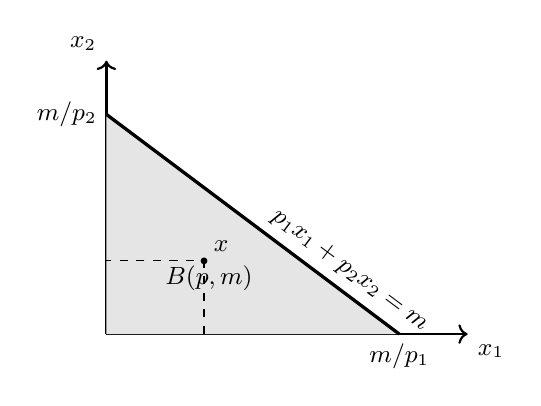
\begin{tikzpicture}[scale=0.62]
  \draw[->,thick] (0,0) -- (7.4,0) node[below right] {\small $x_1$};
  \draw[->,thick] (0,0) -- (0,5.6) node[above left] {\small $x_2$};
  % 预算集阴影
  \fill[gray!20] (0,0) -- (6,0) -- (0,4.5) -- cycle;
  \draw[very thick] (6,0) -- (0,4.5) node[midway,above right,sloped] {\small $p_1x_1+p_2x_2=m$};
  \node[below] at (6,0) {\small $m/p_1$};
  \node[left] at (0,4.5) {\small $m/p_2$};
  \node at (2.1,1.15) {\small $B(p,m)$};
  \draw[dashed] (2,0) -- (2,1.5) -- (0,1.5);
  \fill (2,1.5) circle (2pt) node[above right] {\small $x$};
\end{tikzpicture}
\end{document}
